\documentclass[a4paper, 12pt]{article}

\usepackage[english, russian]{babel}
\usepackage[T2A]{fontenc}
\usepackage[utf8]{inputenc}
\usepackage{mathtext}
\usepackage{amsfonts}
\usepackage{ amssymb }
\usepackage{amsmath}
\usepackage{graphics}
\usepackage{graphicx}
\usepackage{wrapfig}
\usepackage{hyperref}
\usepackage{geometry}
\usepackage{float}
\geometry{
        a4paper,
        total={170mm, 257mm},
        left=20mm,
        top=10mm}

\title{Лабораторная работа 24. \\ Безынерционные линейные цепи}
\author{Балдин Виктор}
\date{\today}
\usepackage{float}
\begin{document}
\maketitle

\section{Делитель напряжения}
\begin{figure}[h]
  \centering
  \includegraphics[width=\textwidth]{delu.png}
  \caption{Делитель напряжения}
\end{figure}

Напряжение $E^{*}$, до которого мы понижаем исходное делителем по этой схеме:
\begin{equation}
  E^{*} = E\frac{R_2}{R_1 + R_2}
\end{equation}

Отсюда
\[ R_2 = R_1\frac{E^{*}}{E - E^{*}} \]

В работе $E=10$ В, $E^{*}=2$ В, $R_1 = 12$ кОм $\Rightarrow R_2 = 3$ кОм.
Соберем схему на макетной плате и измерим напряжение на делителе.
Получили $E^{*} = 1.94$ В.

Измерим сопротивление делителя методом двух нагрузок. В качестве второй нагрузки
возьмем $R_l = 1$ кОм. $U_l = 0.55$ В.
\begin{equation}
  \frac{E^{*} - U_l}{R^*} = \frac{U_l}{R_l}
  \label{2nagr}
\end{equation}
Отсюда $R^* = 2.40$ кОм.

Для переменного тока $e_A = 1.0$ В, $U_A = 180.5$ мВ.
\[ k = \frac{U_A}{e_A} = 0.18 \]

\newpage

\section{Параллельный сумматор}
\begin{figure}[h]
  \centering
  \includegraphics[width=\textwidth]{parsum.png}
  \caption{Параллельный сумматор}
\end{figure}

Некоторые формулы:
\[ \alpha = \frac{R \| R_2}{R_1 + R \| R_2} \]
\[ \beta  = \frac{R \| R_1}{R_2 + R \| R_1} \]
\[ \frac{\alpha}{\beta} = \frac{R_2}{R_1}   \]
\[ \alpha + \beta = \frac{1}{1 + \frac{1}{R_1 \| R_2}} \]

Нам задали весовые коэффициенты $\alpha = 0.4$,
$\beta = 0.2 \Rightarrow \frac{R_2}{R_1} = 2$, $\frac{R}{R_1 \| R_2} = \frac{3}{2}$.

Возьмем $R_1 = 1$ кОм, $R_2 = 2$ кОм, $R = 1$ кОм. Подадим в качестве $E_1$
переменное синусоидальное напряжение с генератора с амплитудой 2 В,
в качестве $E_2$ -- постоянное 5 В.
По очереди включаем оба источника и смотрим сигнал осциллографом.

Получили $\alpha E_1 = 0.774$ В, $\beta E_2 = 0.980$ В
$\Rightarrow \alpha = 0.387$, $\beta = 0.196$.

По методу двух нагрузок: $R_l = 2$ кОм. Подключим $E_1 = E_2 = 5$ В. $E^* = 3.1011$ В.
$U_l = 2.4122$. Отсюда по формуле \ref{2nagr} $R^* = 0.57$ кОм.

Результат близок к теоретической оценке $R^* = R_1 \| R_2 \| R = 0.5$ кОм.

\newpage

\section{$H$-параметры}
\begin{figure}[h]
  \centering
  \includegraphics[width=0.5\textwidth]{t-scheme.png}
  \caption{Т-образная схема}
\end{figure}

Проверим формулы для $H$ - параметров $T$-образной схемы:
\begin{equation}
  \begin{pmatrix}
    U_1 \\
    I_2
  \end{pmatrix}
  =
  \begin{pmatrix}
    h_{11} & h_{12} \\
    h_{21} & h_{22}
  \end{pmatrix}
  \begin{pmatrix}
    I_1\\
    U_2
  \end{pmatrix}
  =
  \begin{pmatrix}
    R_1 + R_3 \| R_2 & \frac{R_3}{R_3 + R_2} \\
    -\frac{R_3}{R_3 + R_2} & \frac{1}{R_3 + R_2}
  \end{pmatrix}
  \begin{pmatrix}
    I_1 \\
    U_2
  \end{pmatrix}
  \label{eq:hpar}
\end{equation}

Открываем в Micro-Cap файл \texttt{hpar.cir}. Запускаем измерения. Снимок экрана
на рис. \ref{hpar}. По результатам измерений:
\begin{align*}
  h_{11} = \frac{U_1}{I_1} = 2.2\ \text{кОм} &,\ h_{12} = \frac{U_1}{U_2} = 0.6\\
  h_{21} = \frac{I_2}{I_1} = -0.6&,\ h_{22} = \frac{I_2}{U_2} = 2\cdot10^{-4}\ \text{Ом}^{-1}
\end{align*}

Формула \ref{eq:hpar} подтвердилась.

\section{$X$-параметры}
Проверим формулы для $X$-параметров:
\begin{equation}
  \begin{pmatrix}
    U_1 \\
    U_2
  \end{pmatrix}
  =
  \begin{pmatrix}
    X_{11} & X_{12} \\
    X_{21} & X_{22}
  \end{pmatrix}
  \begin{pmatrix}
    I_1\\
    I_2
  \end{pmatrix}
  =
  \begin{pmatrix}
    R_1 + R_3 & R_3 \\
    R_3 & R_2 + R_3
  \end{pmatrix}
  \begin{pmatrix}
    I_1 \\
    I_2
  \end{pmatrix}
  \label{eq:xpar}
\end{equation}

Откроем файл \texttt{xpar.cir}. Пересчитаем представленные там параметры звезды
в параметры треугольника:
\begin{eqnarray*}
  R_{13} = R_1 + R_3 + \frac{R_1R_3}{R_2} = 5.5\ \text{кОм}\\
  R_{12} = R_1 + R_2 + \frac{R_1R_2}{R_3} = 3.67\ \text{кОм}\\
  R_{23} = R_2 + R_3 + \frac{R_2R_3}{R_1} = 11\ \text{кОм}
\end{eqnarray*}

Результаты:
\begin{align*}
  X_{11} = \frac{U_1}{I_1} = 4\ \text{кОм}, &\ X_{12} = \frac{U_1}{I_2} = 3\ \text{кОм}\\
  X_{21} = \frac{U_2}{I_1} = 3\ \text{кОм}, &\ X_{22} = \frac{U_2}{I_2} = 5\ \text{кОм}
\end{align*}

Результаты подтверждают формулу.

\newpage
\section{Лестничные структуры}
\begin{figure}[h]
  \centering
  \includegraphics[width=\textwidth]{apar.png}
  \caption{Лестничная структура}
\end{figure}

Передаточная матрица лестничной структуры с резисторами $R_1 = 1$ и $R_2 = \alpha$:

\begin{equation}
  \begin{pmatrix}
    U_2 \\
    I_2
  \end{pmatrix}
  =
  \begin{pmatrix}
    A_{11} & A_{12} \\
    A_{21} & A_{22}
  \end{pmatrix}
  \begin{pmatrix}
    U_1\\
    I_1
  \end{pmatrix}
  =
  \begin{pmatrix}
    1 & -1 \\
    -\frac{1}{\alpha} & \frac{1+\alpha}{\alpha}
  \end{pmatrix}
  \begin{pmatrix}
    U_1 \\
    I_1
  \end{pmatrix}
  \label{eq:apar}
\end{equation}

Откроем файл \texttt{apar.cir}. Результаты измерений при $\alpha = 2, 6, 12, 1$
и $\gamma = \frac{1}{2}, \frac{2}{3}, \frac{3}{4}, \frac{\sqrt{5} - 1}{\sqrt{5} + 1}$
приведены на снимках экрана в конце отчета.

Откроем файл \texttt{dac.cir} со схемой 4-разрядного ЦАП, который преобразует двоичный
код в напряжение по формуле
\begin{equation}
  OUT = X_32^3 + X_22^3 + X_12^1 + X_0
\end{equation}

Проведя измерения в Micro-Cap 16 раз для всех двоичных кодов, получим зависимость
$OUT(X_3, X_2, X_1, X_0)$:
\begin{table}[h]
  \centering
  \begin{tabular}{|c|c|}
    \hline
    $(X_3, X_2, X_1, X_0)$ & $OUT$ \\ \hline
    0000 & 0 \\ \hline
    0001 & 1 \\ \hline
    0010 & 2 \\ \hline
    0011 & 3 \\ \hline
    0100 & 4 \\ \hline
    0101 & 5 \\ \hline
    0110 & 6 \\ \hline
    0111 & 7 \\ \hline
    1000 & 8 \\ \hline
    1001 & 9 \\ \hline
    1010 & 10 \\ \hline
    1011 & 11 \\ \hline
    1100 & 12 \\ \hline
    1101 & 13 \\ \hline
    1110 & 14 \\ \hline
    1111 & 15 \\ \hline
  \end{tabular}
\end{table}

\newpage
\section{Вывод}
В ходе работы были подтверждены при помощи компьютерной симуляции теоретические формулы,
выведенные для $H$-, $X$- и $A$- параметров распространенных электрических схем.

\newpage

\begin{figure}
  \centering
  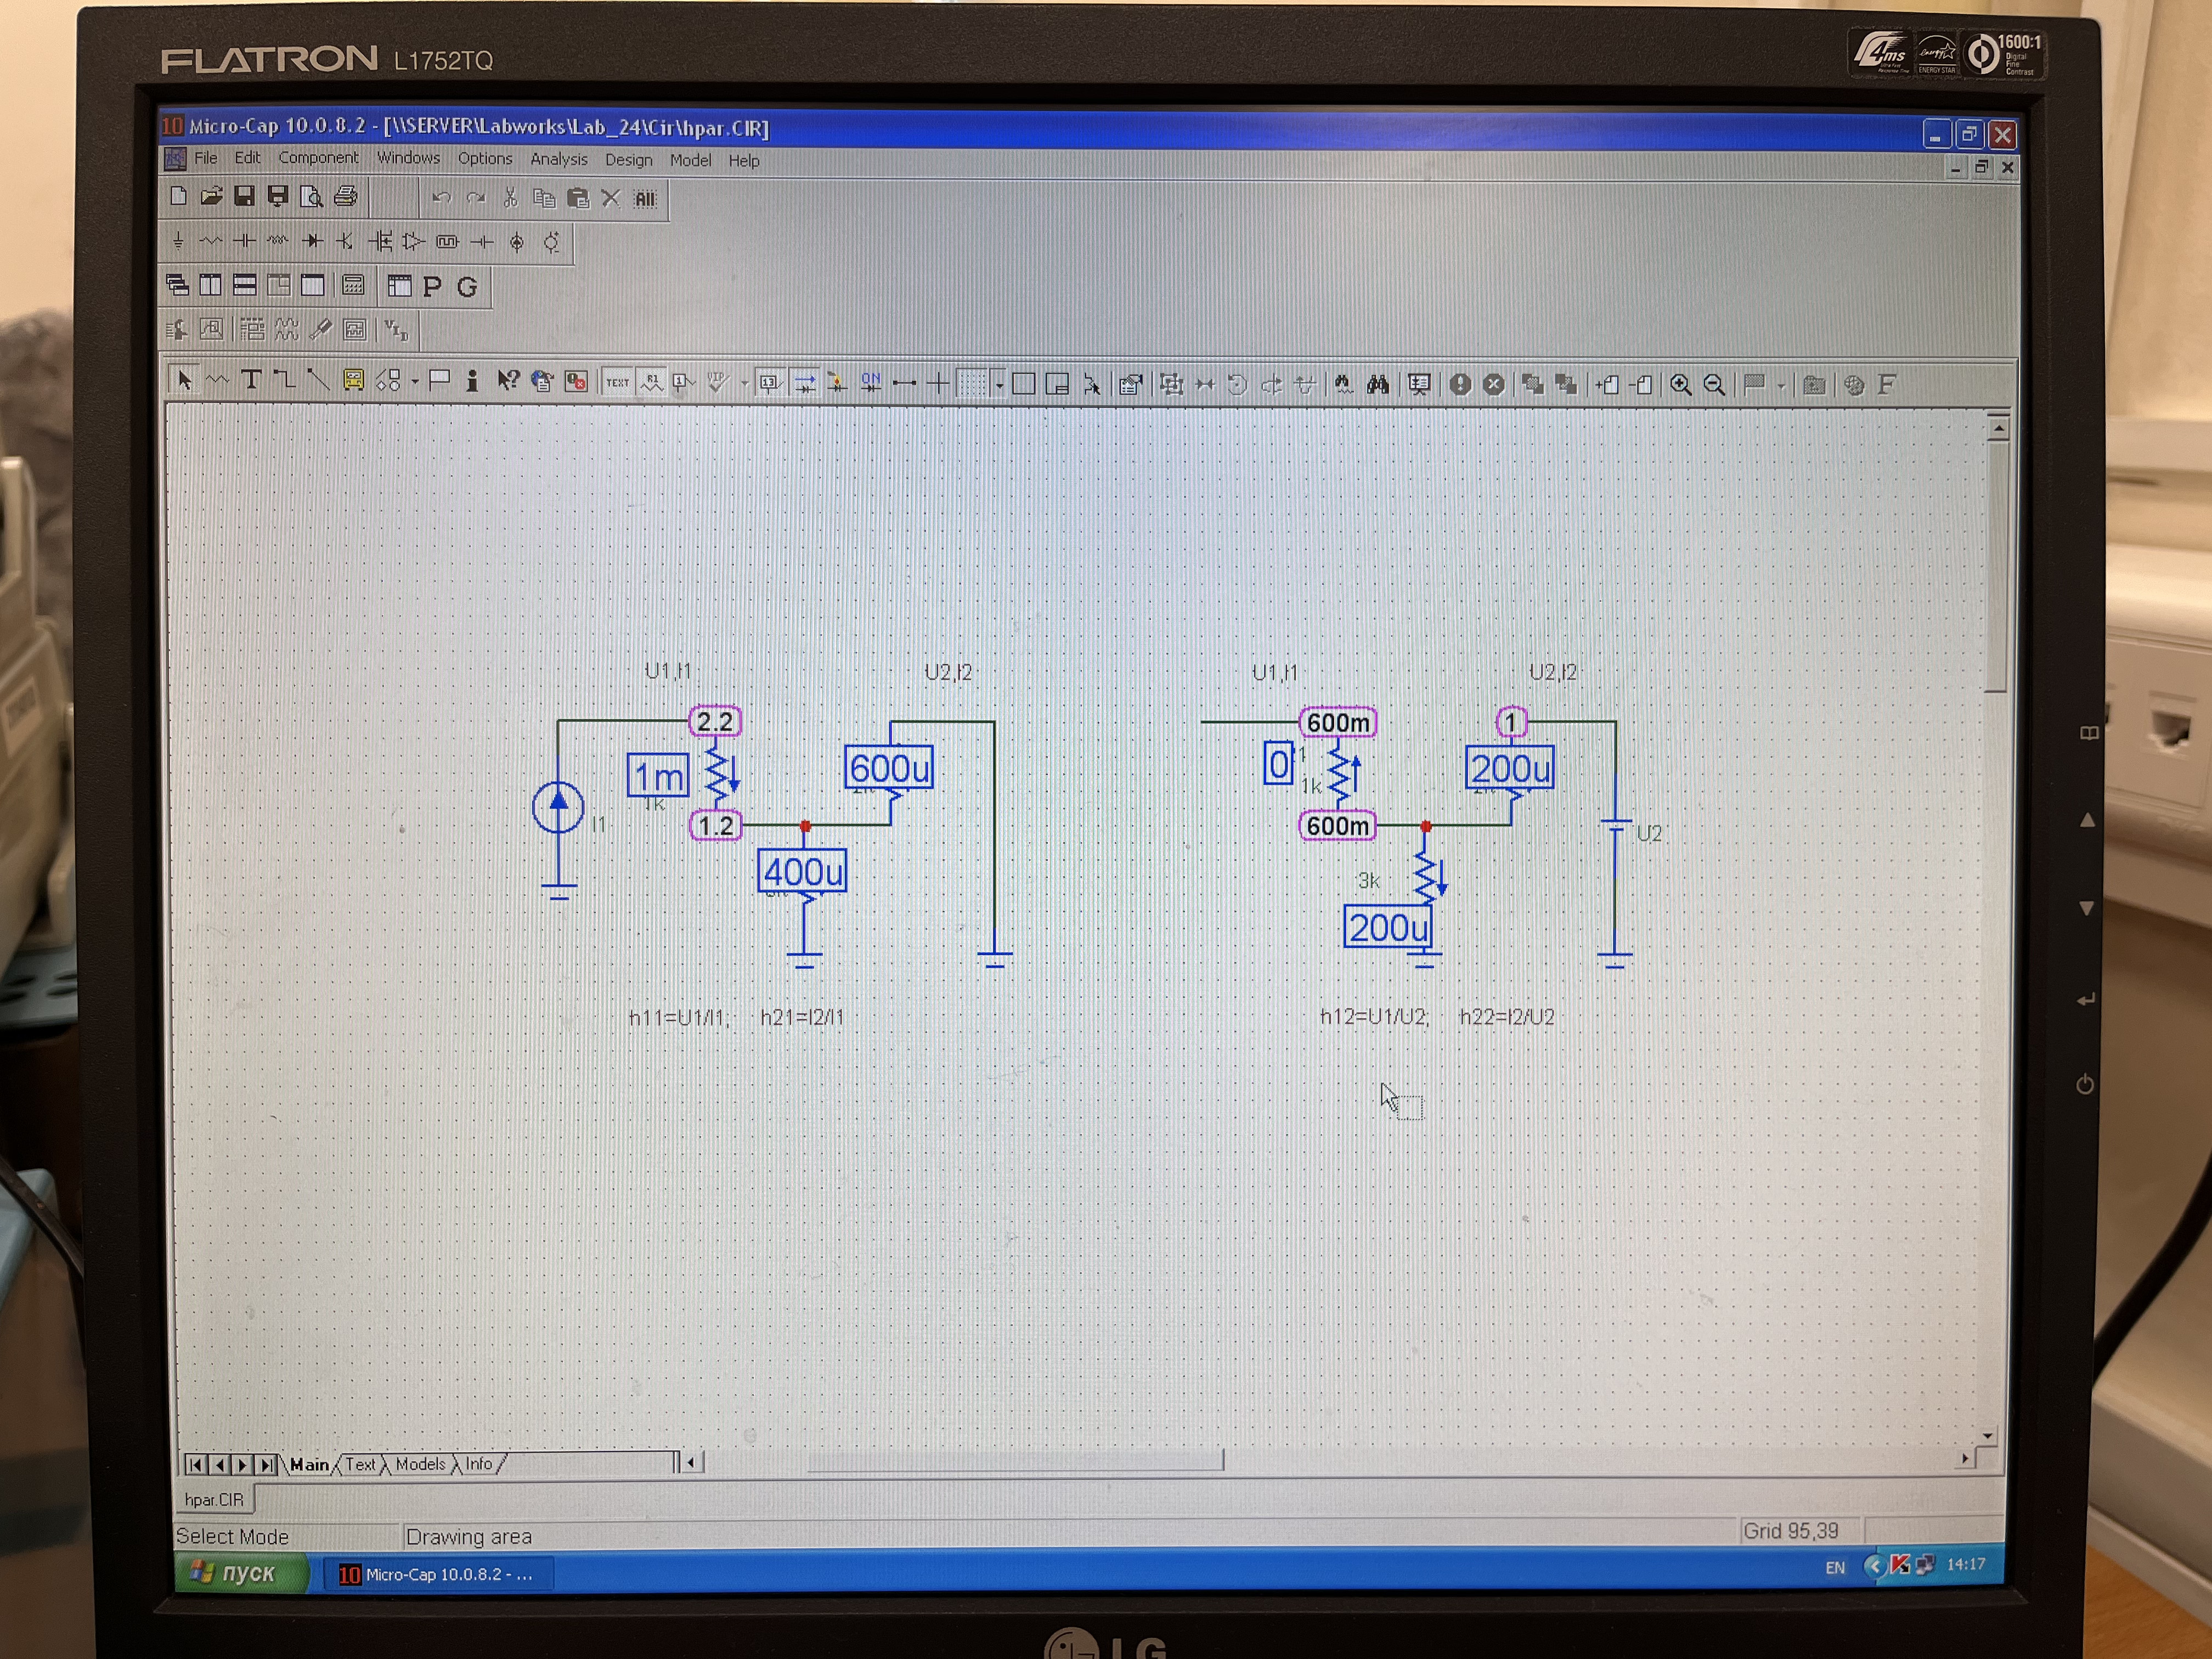
\includegraphics[width=\textwidth]{hpar.jpg}
  \caption{Снимок экрана при измерении $H$- параметров}
  \label{hpar}
\end{figure}

\begin{figure}
  \centering
  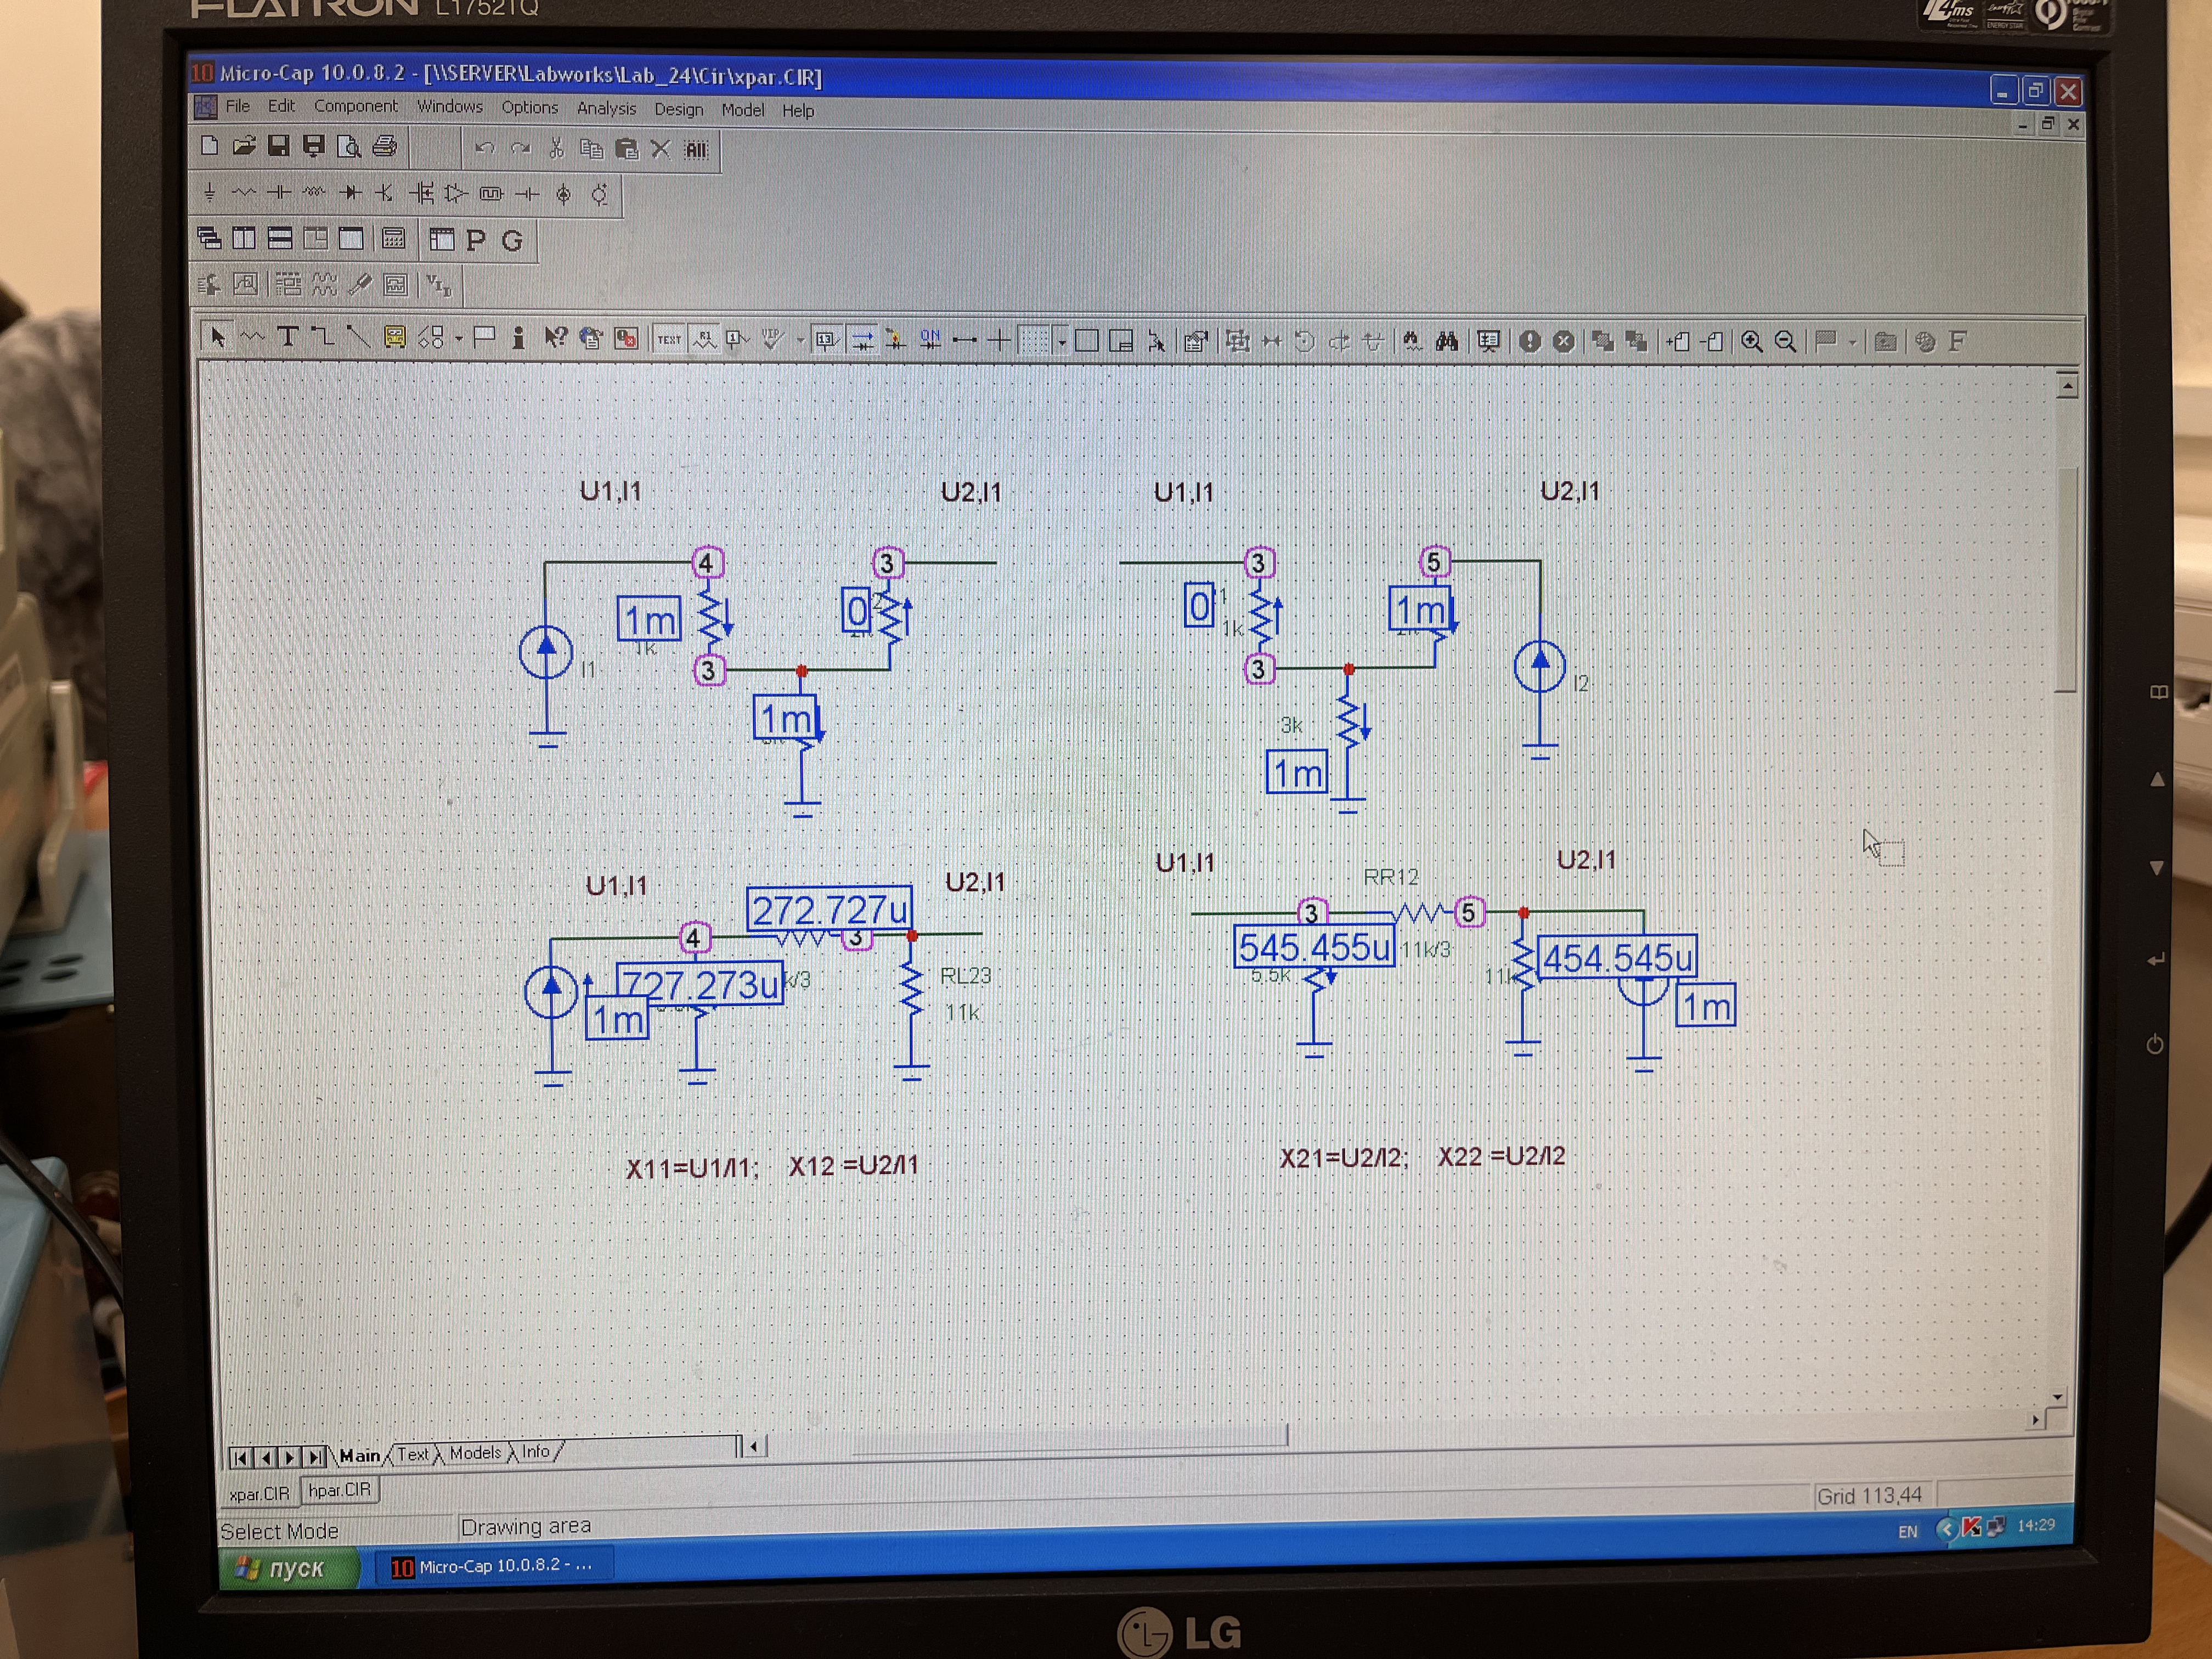
\includegraphics[width=\textwidth]{IMG_2860.jpg}
  \caption{Снимок экрана при измерении $X$-параметров}
  \label{xpar}
\end{figure}

\begin{figure}
  \centering
  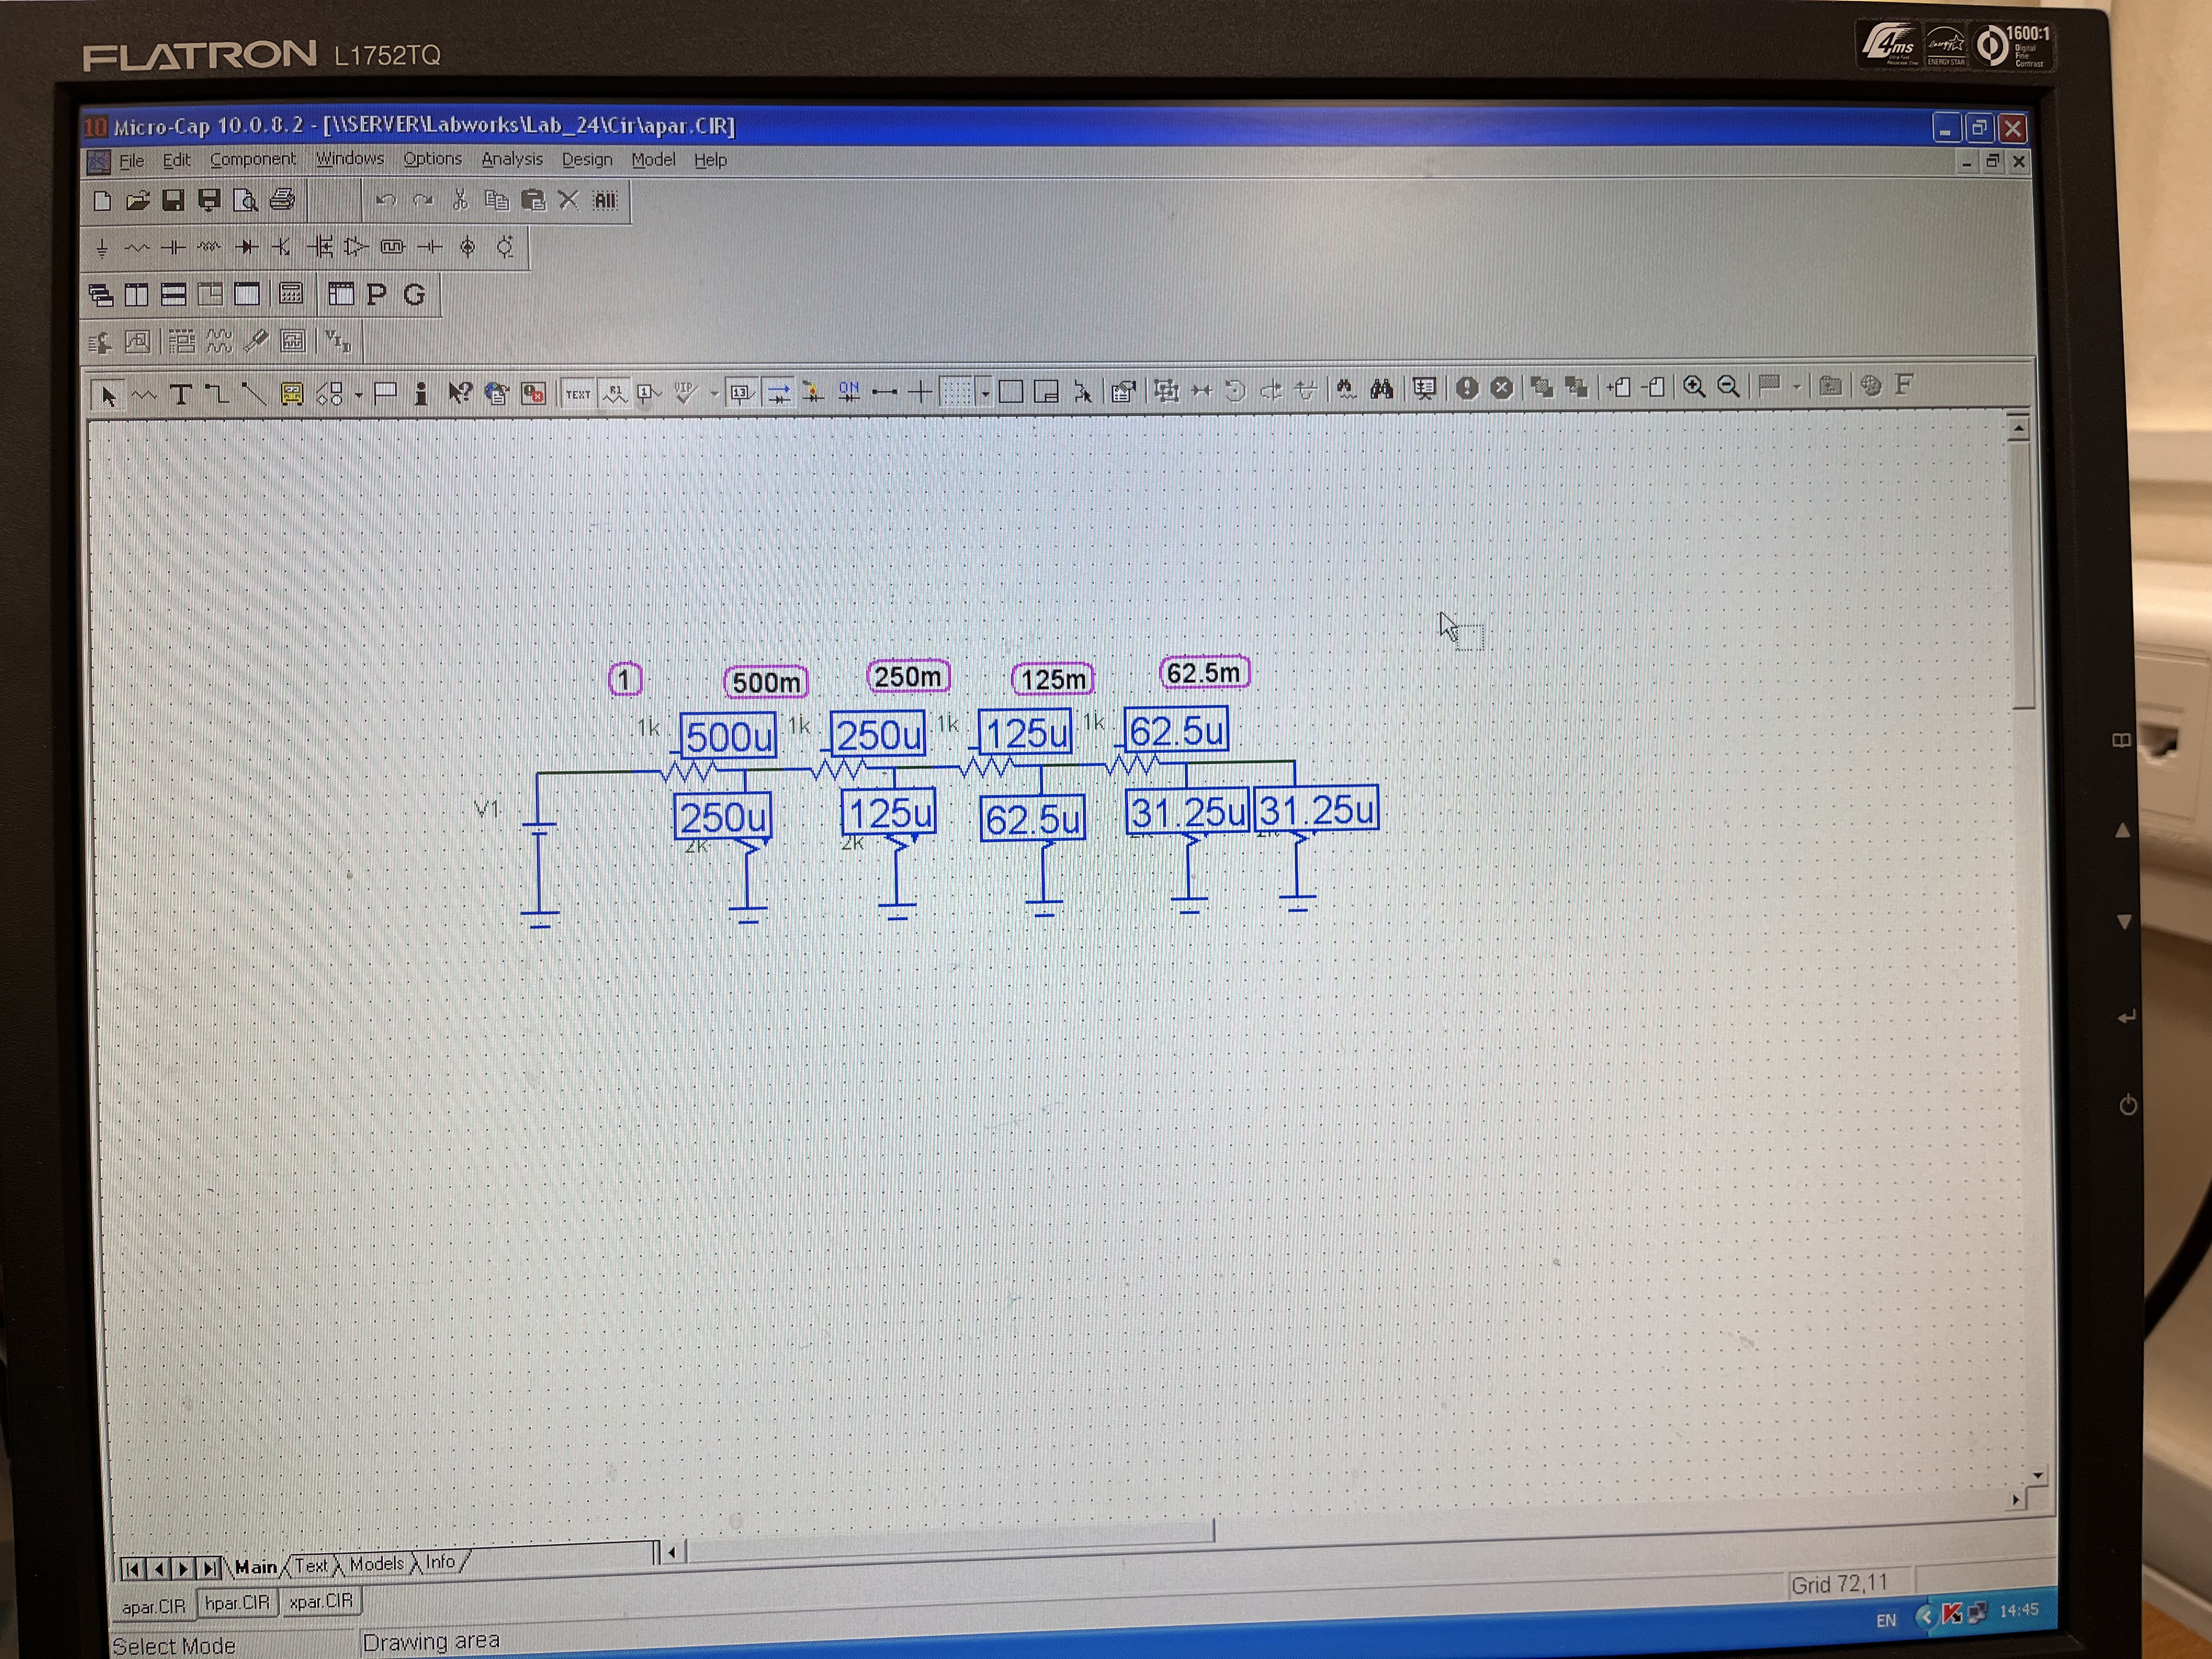
\includegraphics[width=\textwidth]{IMG_2861(1).jpg}
  \caption{Снимок экрана при измерении $A$-параметров для $\alpha = 2$, $\gamma = \frac{1}{2}$}
\end{figure}

\begin{figure}
  \centering
  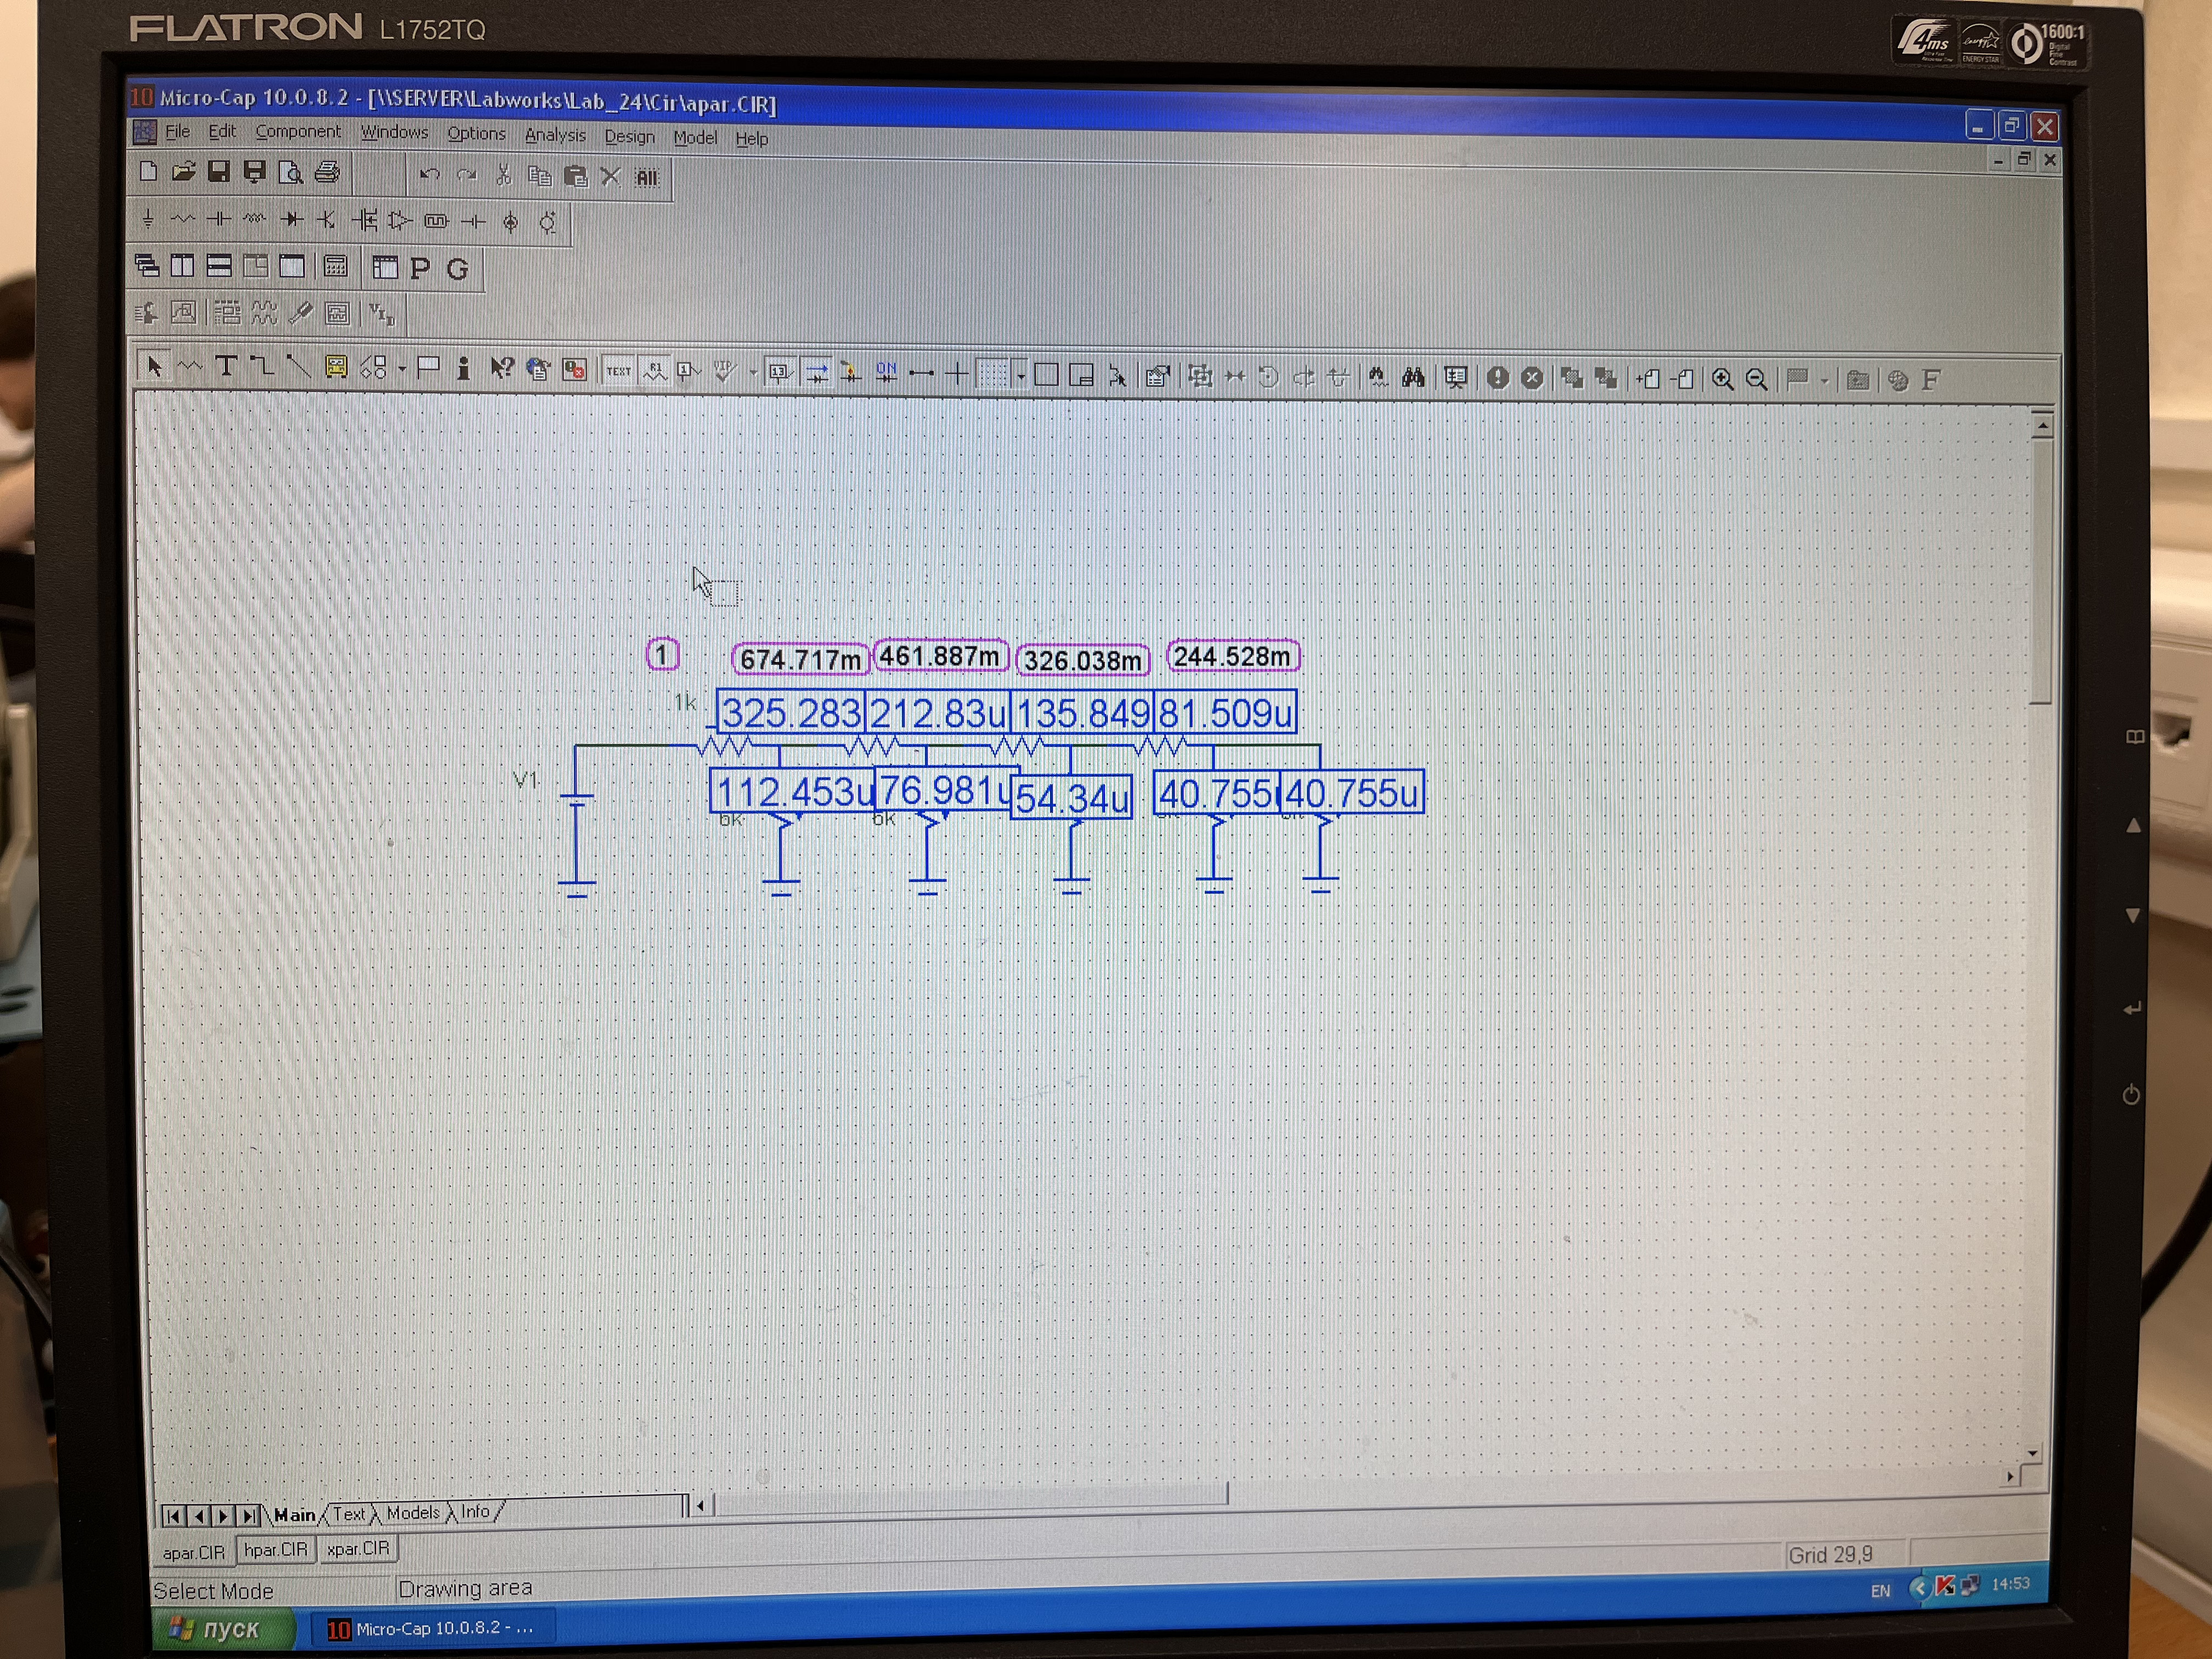
\includegraphics[width=\textwidth]{IMG_2862(1).jpg}
  \caption{Снимок экрана при измерении $A$-параметров для $\alpha = 6$, $\gamma = \frac{2}{3}$}
\end{figure}

\begin{figure}
  \centering
  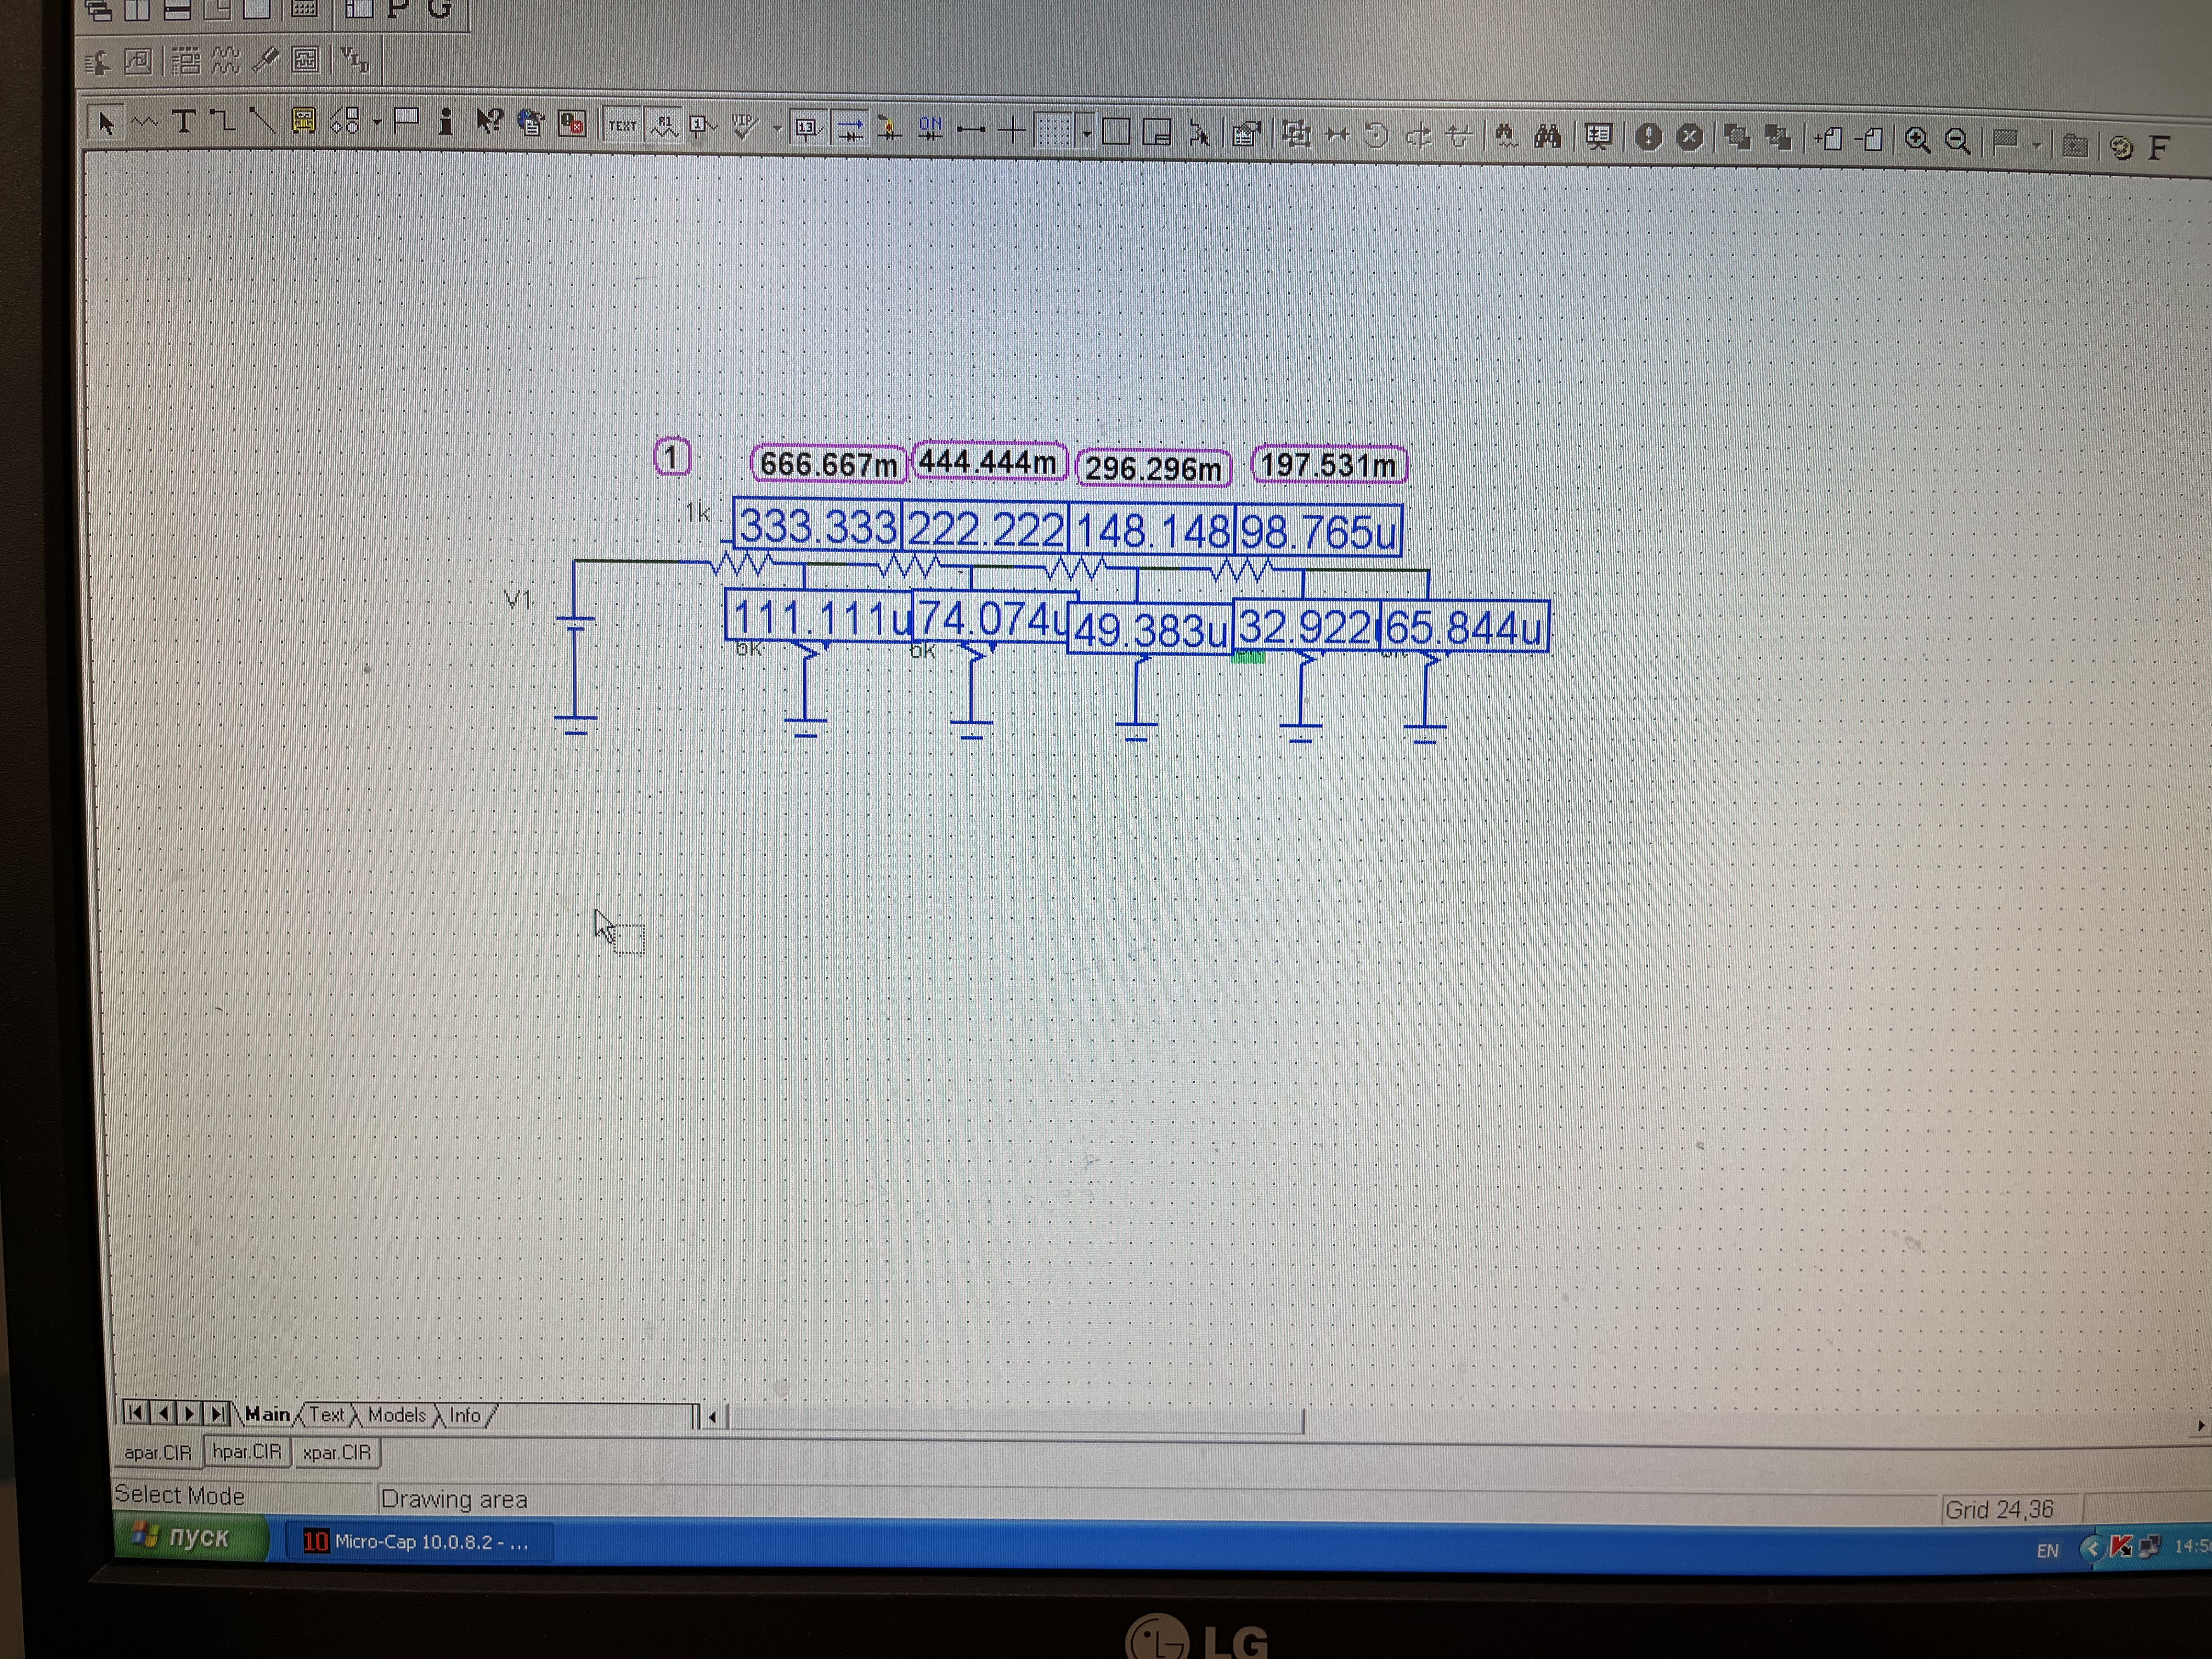
\includegraphics[width=\textwidth]{IMG_2863.jpg}
  \caption{Снимок экрана при измерении $A$-параметров для $\alpha = 12$, $\gamma = \frac{3}{4}$}
\end{figure}

\begin{figure}
  \centering
  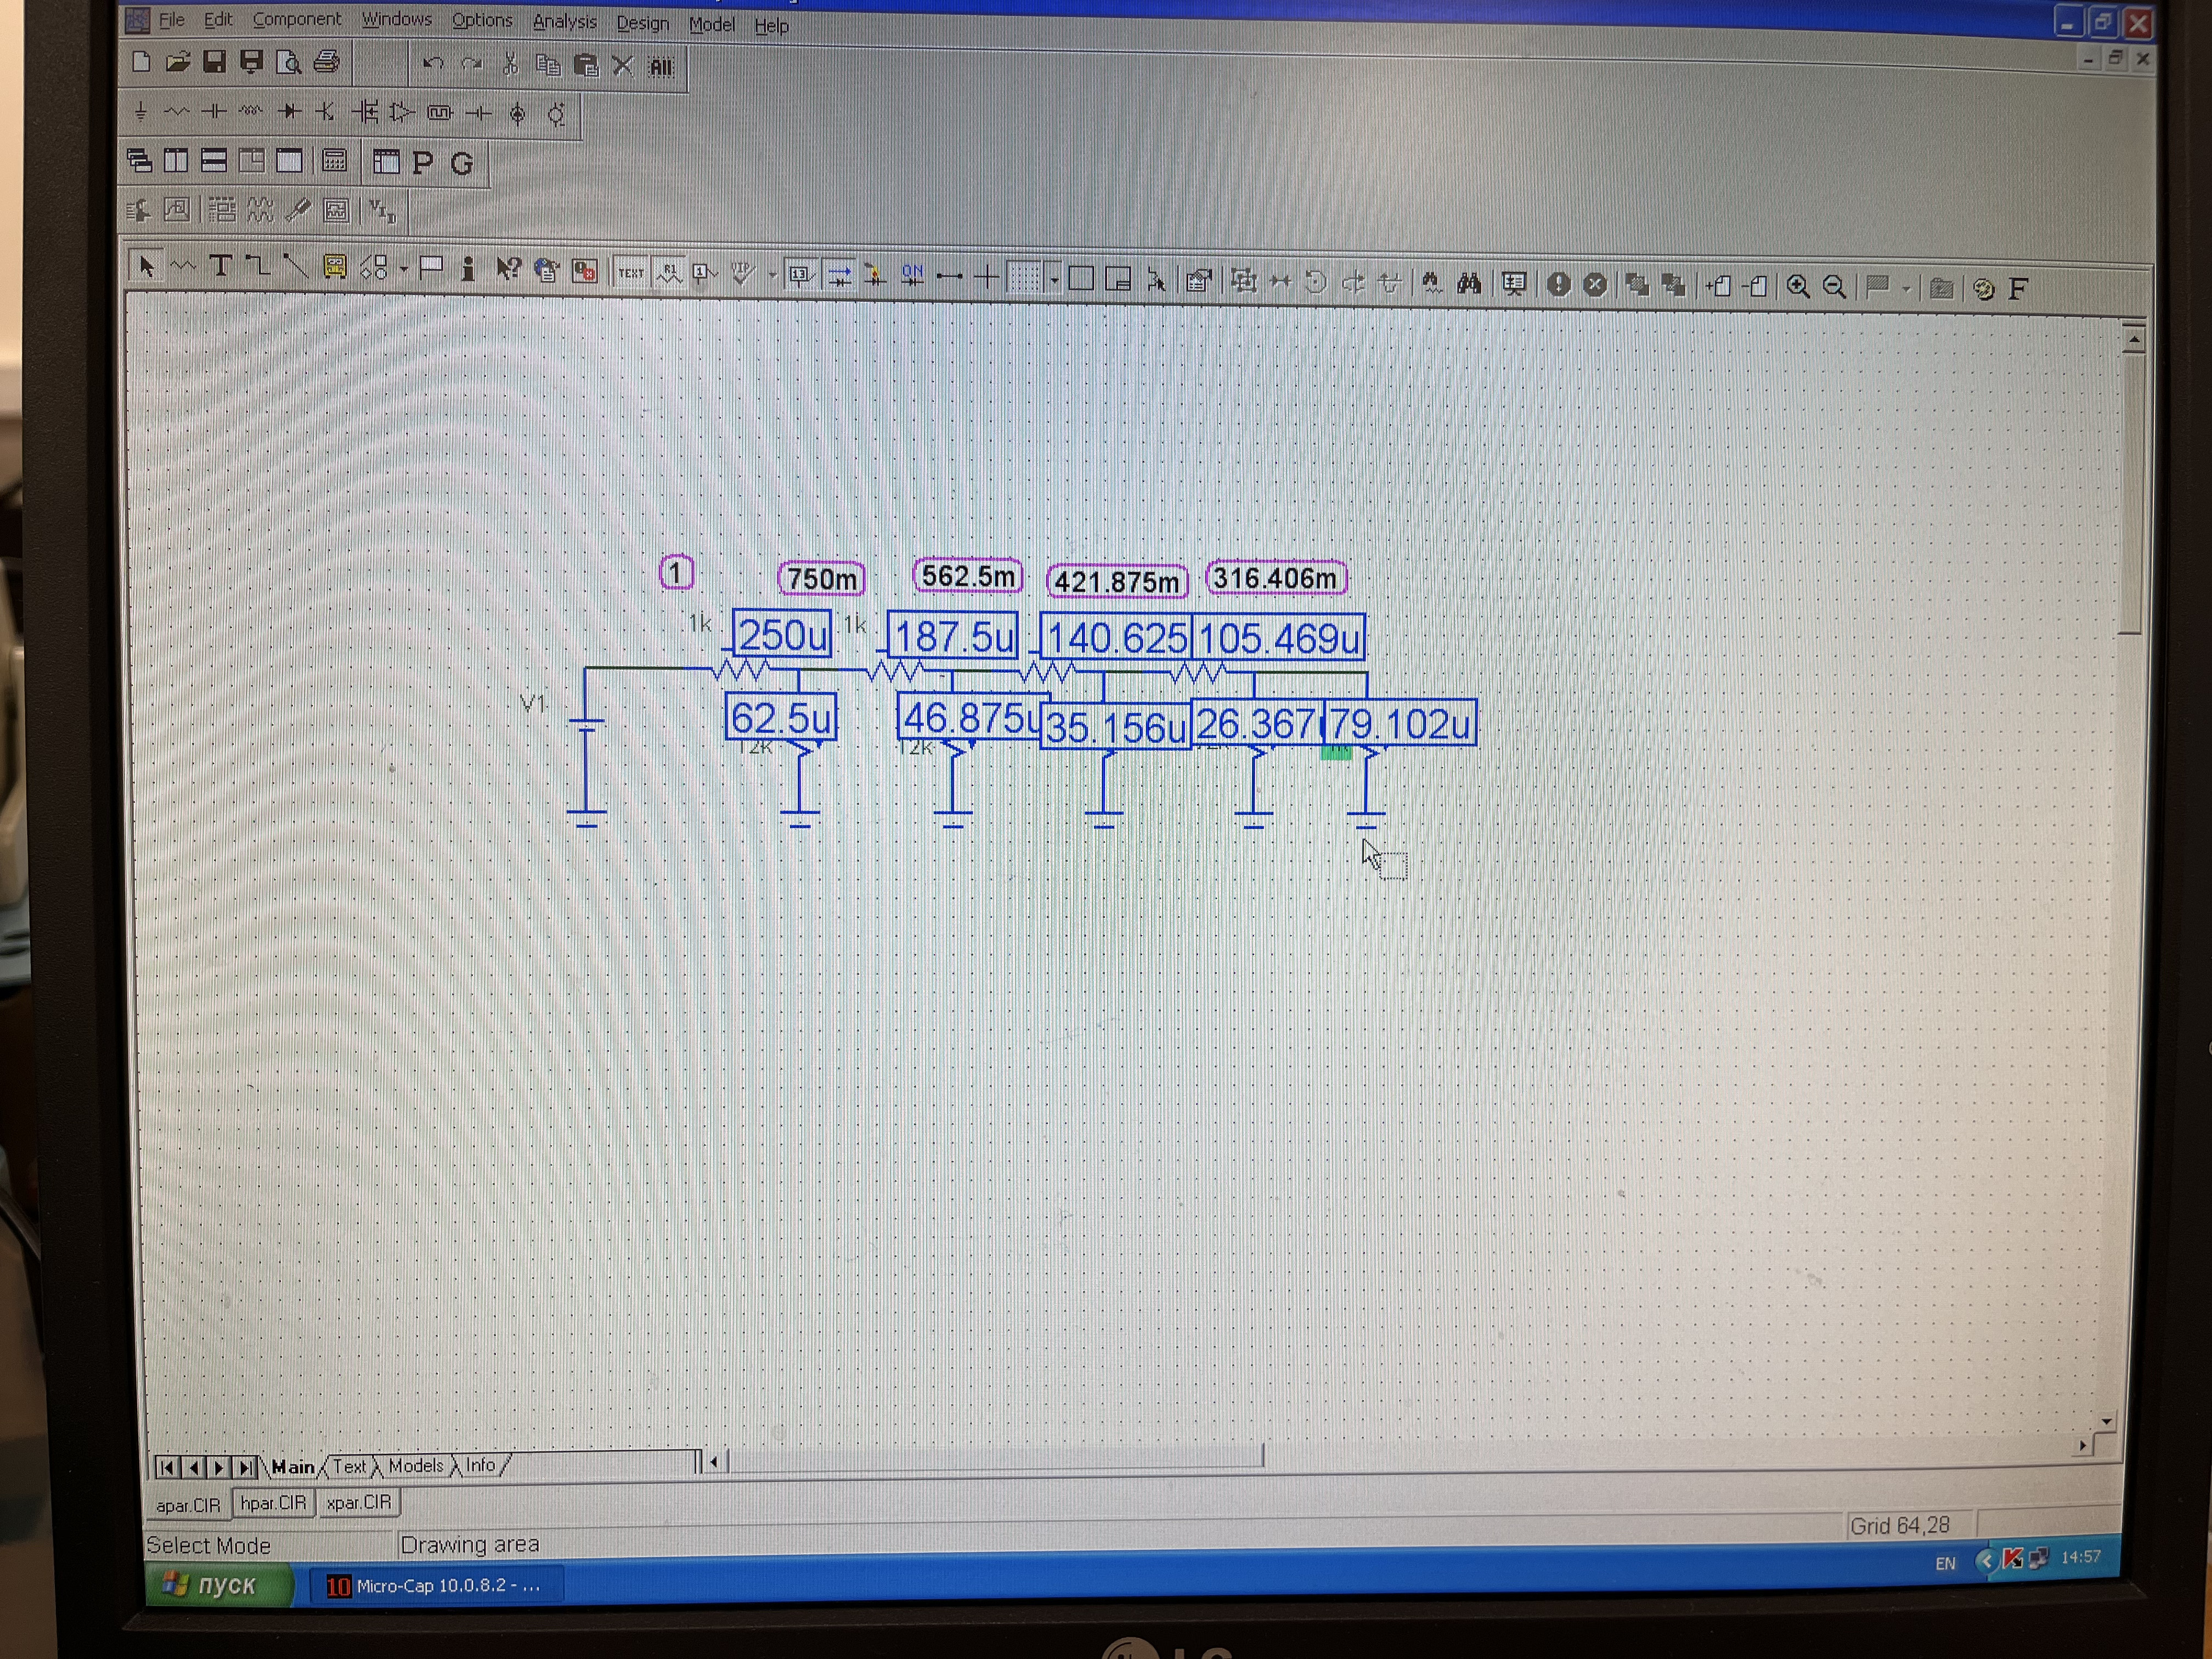
\includegraphics[width=\textwidth]{IMG_2864(1).jpg}
  \caption{Снимок экрана при измерении $A$-параметров для $\alpha = 1$, $\gamma = \frac{\sqrt{5} - 1}{\sqrt{5} + 1}$}
\end{figure}

\begin{figure}
  \centering
  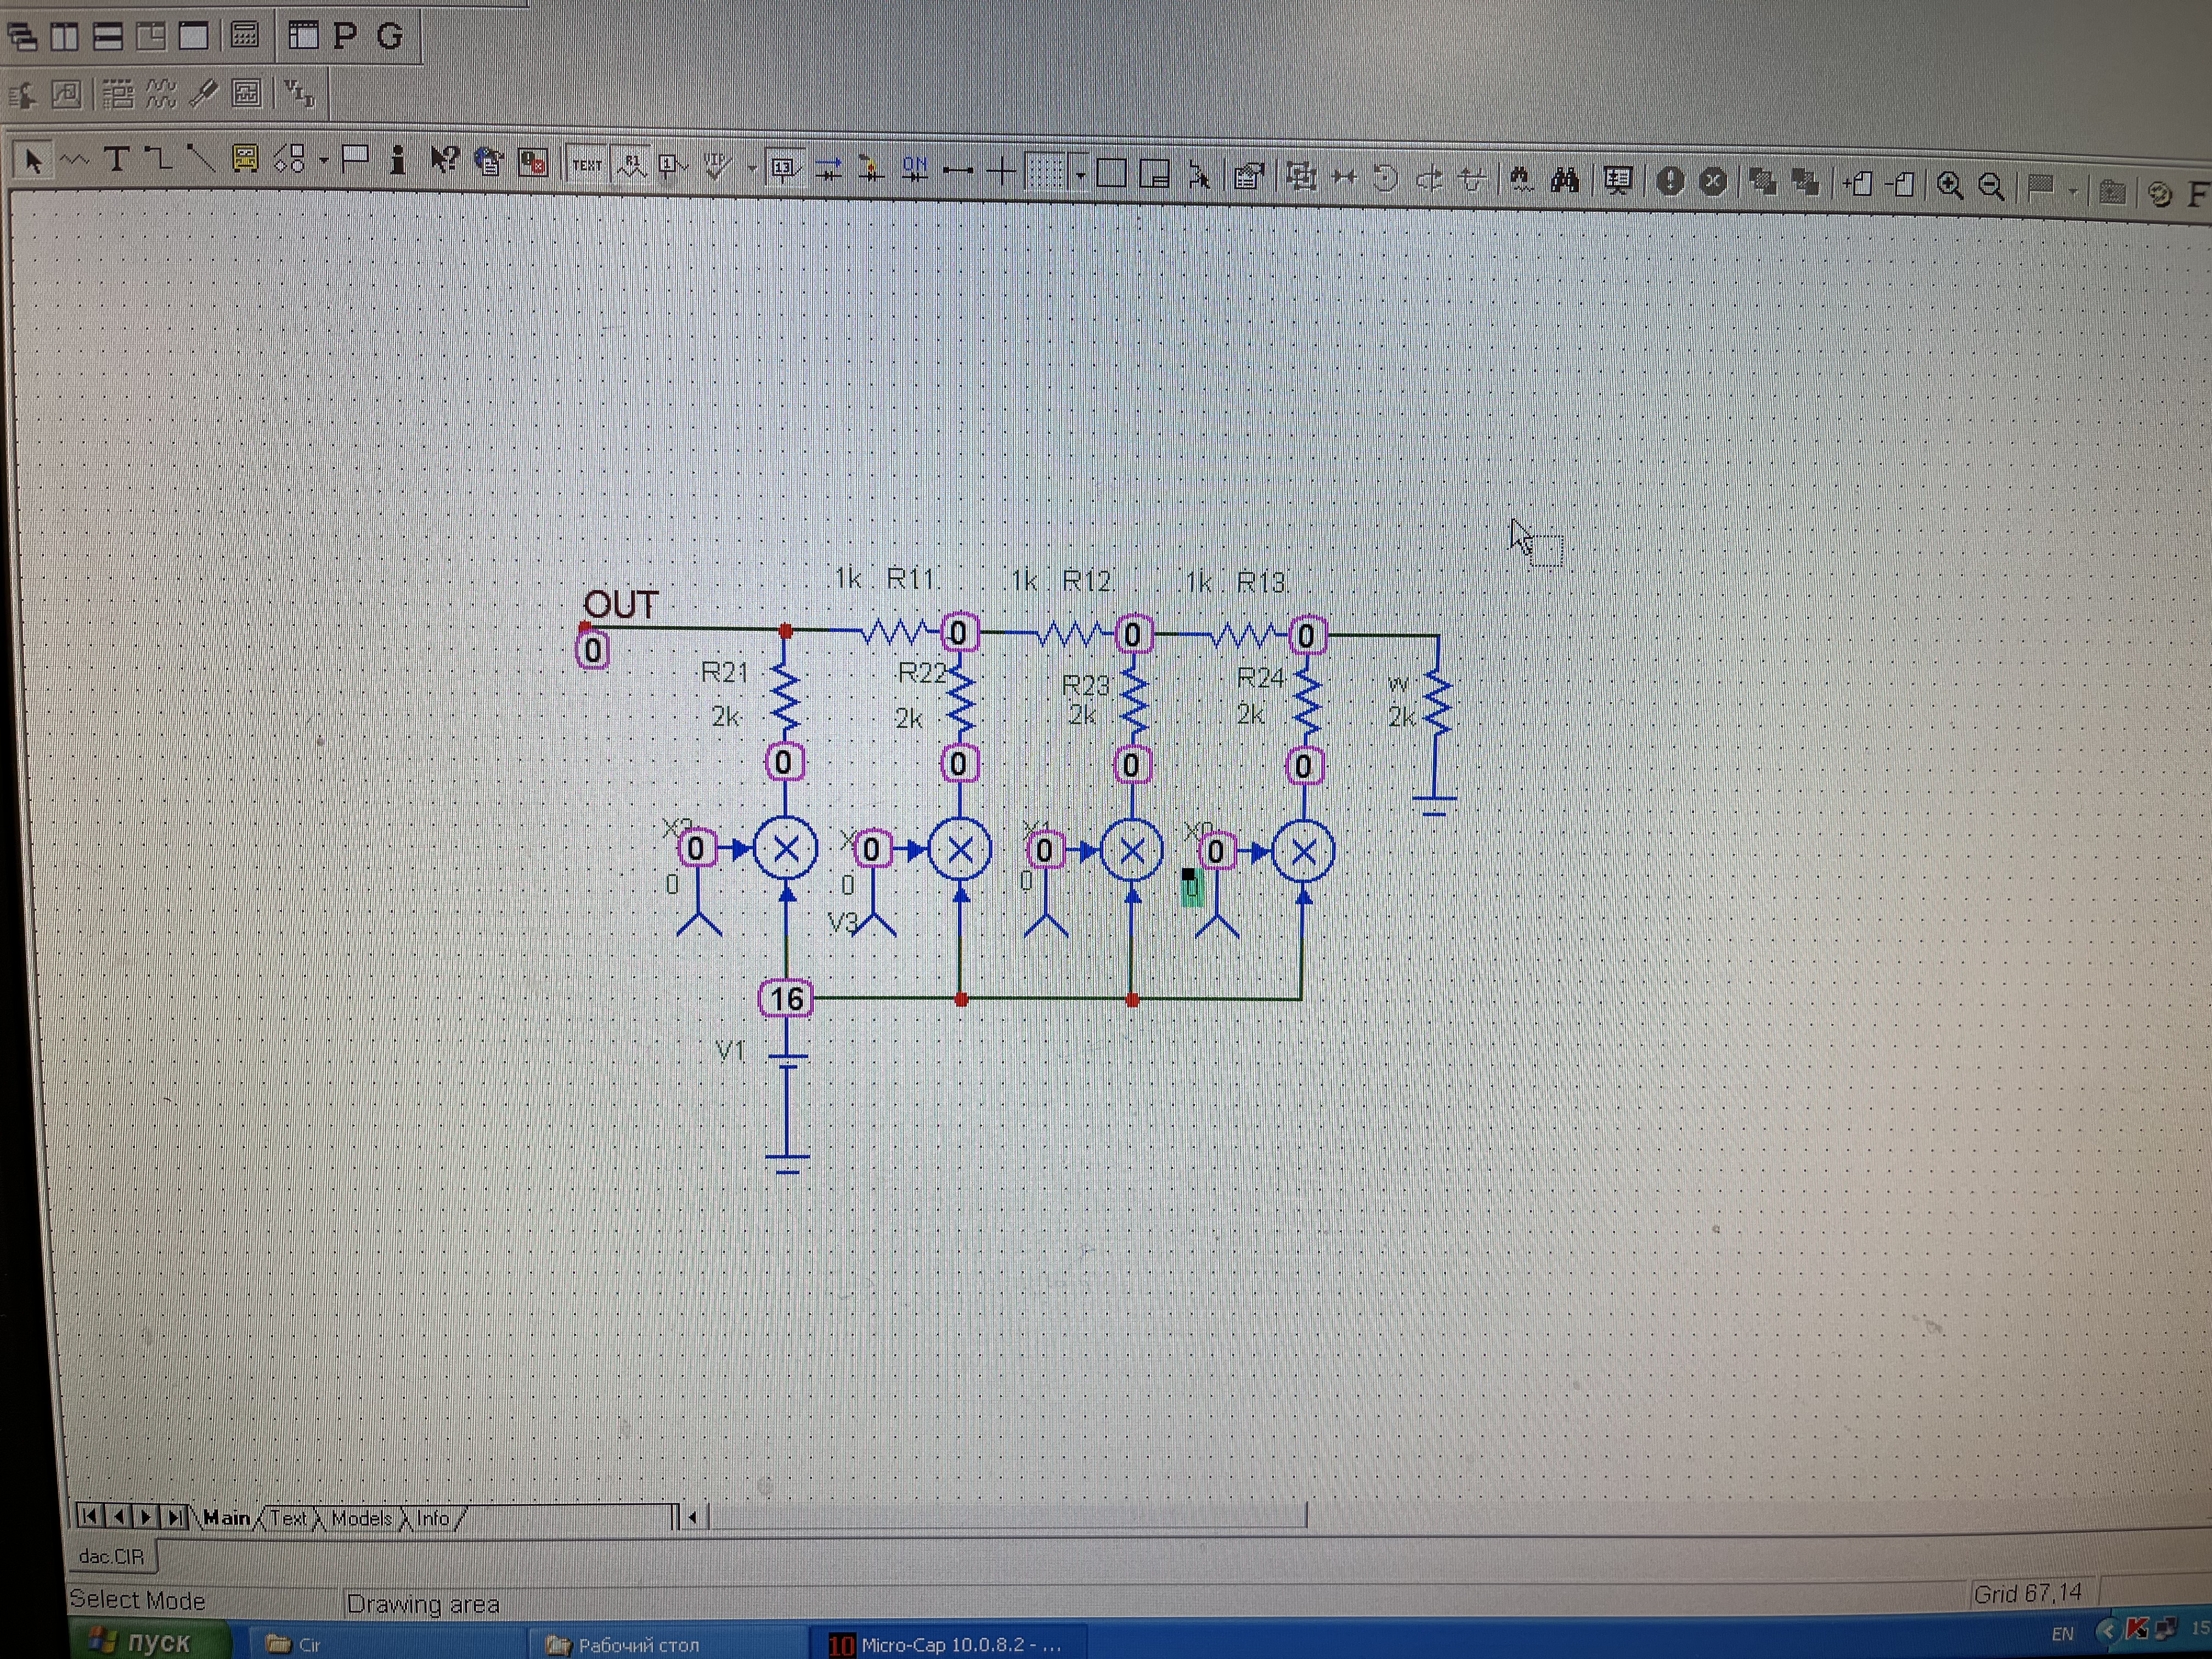
\includegraphics[width=\textwidth]{IMG_2865(1).jpg}
  \caption{Снимок экрана для ЦАП}
\end{figure}

\begin{figure}
  \centering
  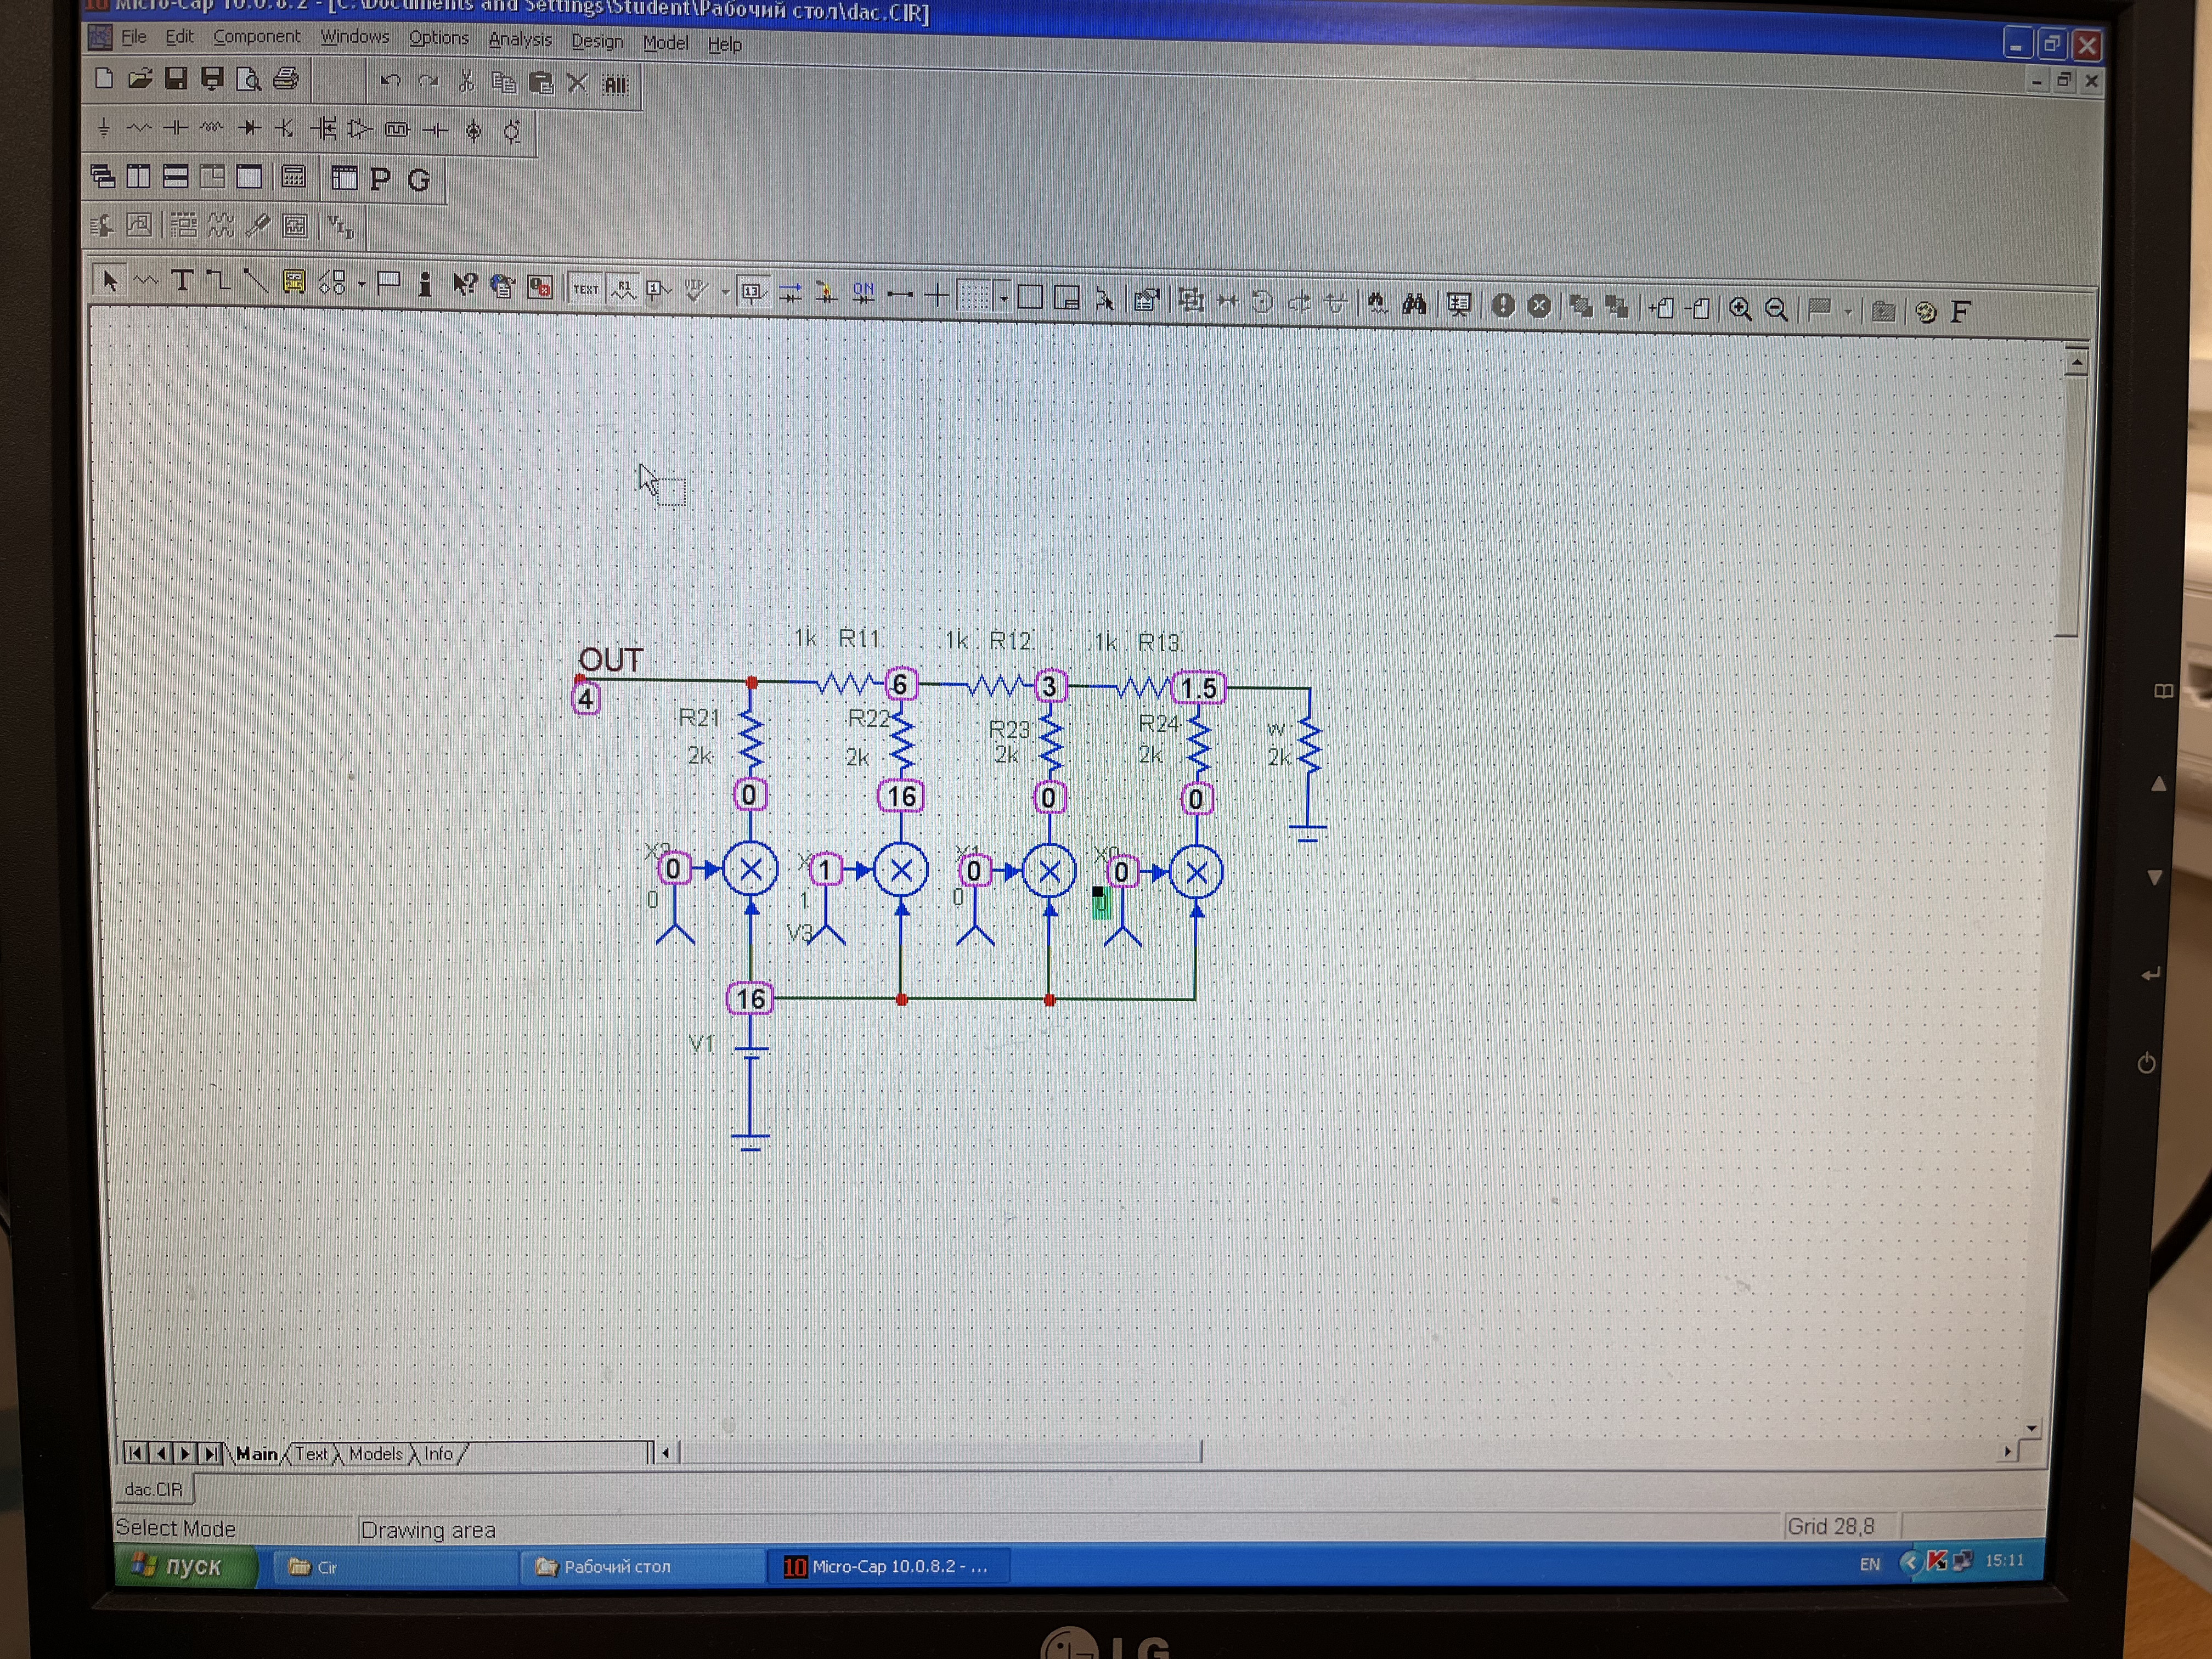
\includegraphics[width=\textwidth]{IMG_2868.jpg}
  \caption{Снимок экрана для ЦАП}
\end{figure}


\end{document}
